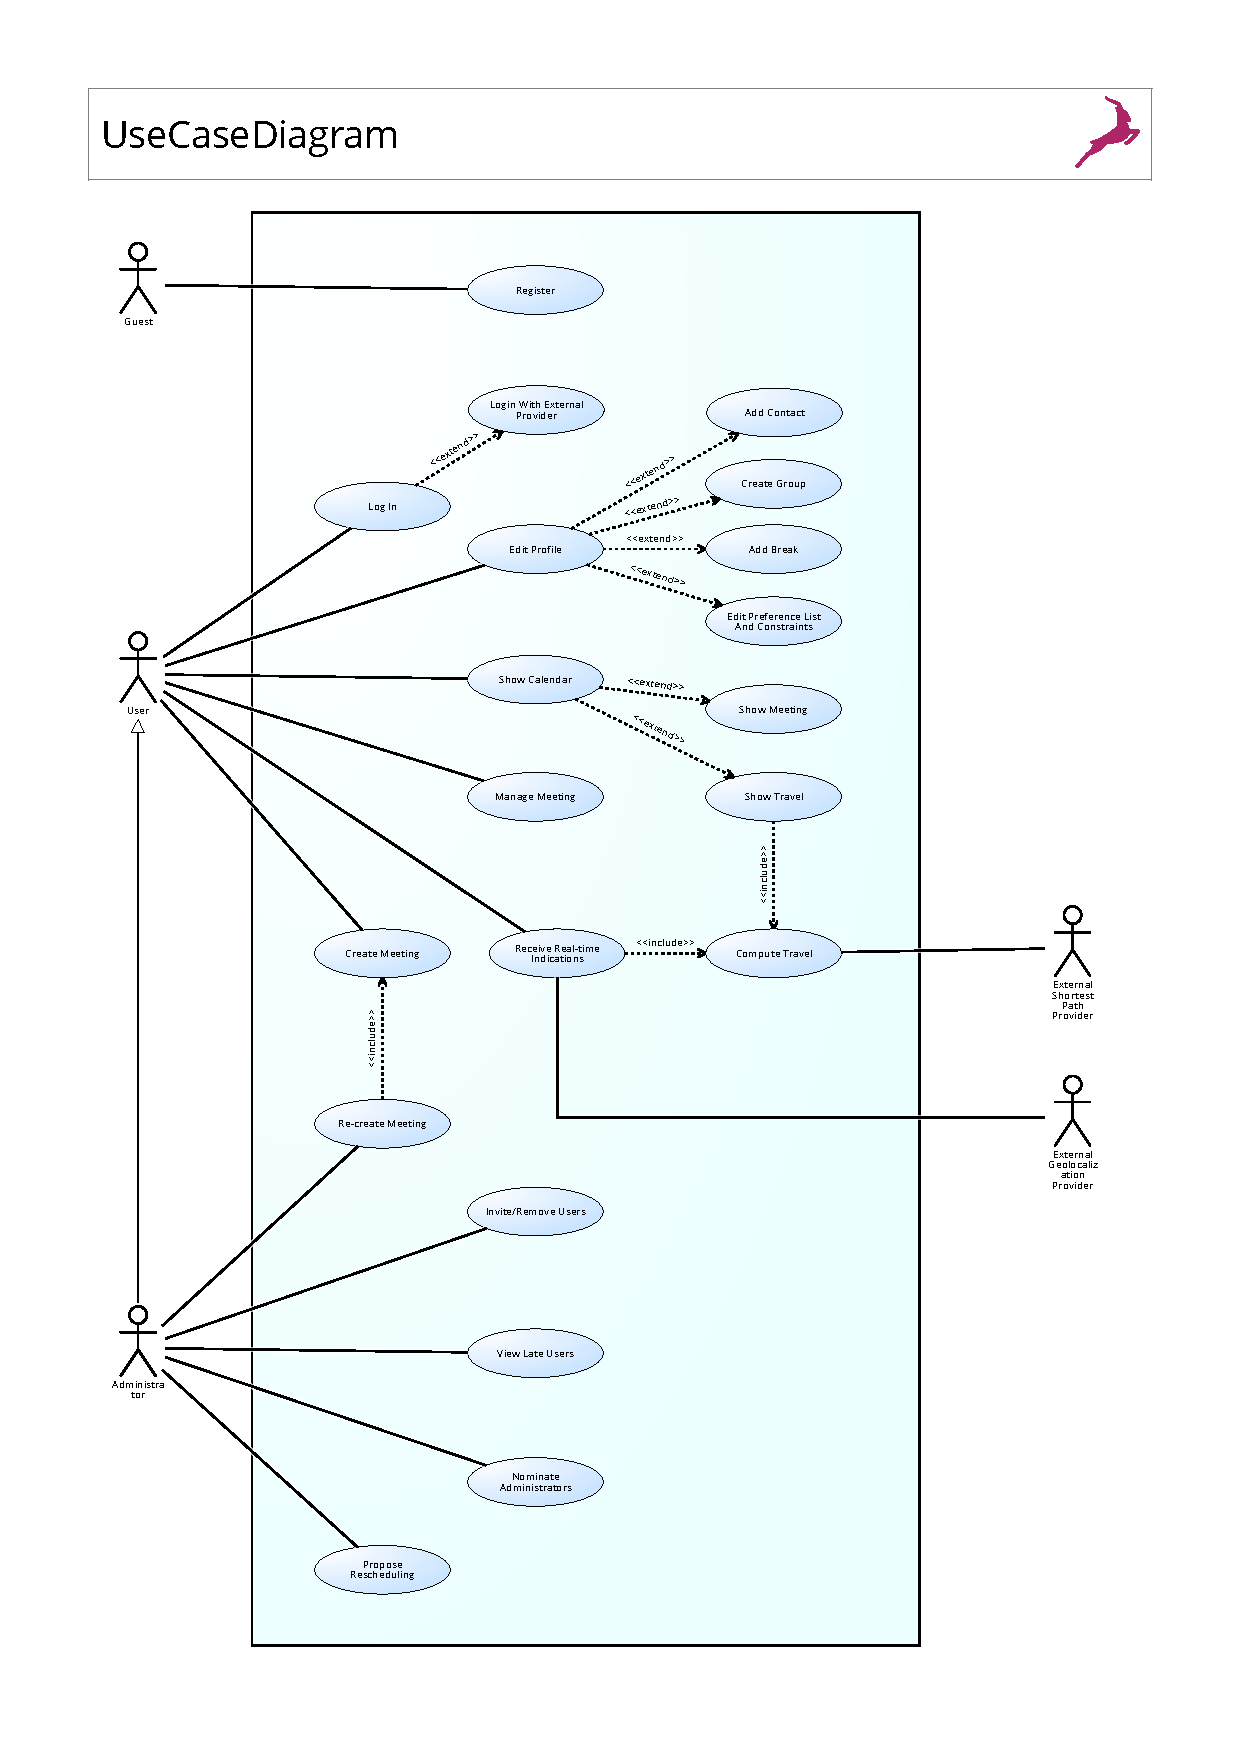
\includepdf[pages=-]{Pdf/UseCaseDiagram.pdf}

\begin{table}[H]
	\centering
	\def\arraystretch{1.5}
	\begin{tabular}{|p{7cm}|p{7cm}|}
		\hline
		\textbf{Actors}            & Guest, External Login Provider		    \\ \hline
		\textbf{Goals}             & G1           \\ \hline
		\textbf{Input Conditions}  & A guest is on the homepage of the system.           \\ \hline
		\textbf{Events Flow}       &   
		Registration via user credentials
		\begin{enumerate}
			\item The guest inserts its main email address.
			\item The guest enters its password.
			\item The guest clicks on the "Sign Up" button.
		\end{enumerate}
		Registration via External Service Provider
		\begin{enumerate}
			\item The guest clicks on the "Log in with \texttt{Service name}" button
			\item The guest is taken to an external page where it has to follow the authentication procedure of the external login provider
			\item The guest is redirected to our system with a valid token
		\end{enumerate}       \\ \hline
		\textbf{Output Conditions} & The guest is registered into the system with a pair \texttt{email - password} or with a token, given by the external provider. The guest becomes a user.          \\ \hline
		\textbf{Exceptions}        & The guest inserts a wrong or already-used email or the external login provider procedure cannot be completed correctly. In either case the system shows the user a message reporting the errors and waits for another attempt.            \\ \hline
	\end{tabular}
	\caption{Register}
\end{table}

\begin{table}[H]
	\centering
	\def\arraystretch{1.5}
	\begin{tabular}{|p{7cm}|p{7cm}|}
		\hline
		\textbf{Actors}            & User, External Login Provider		    \\ \hline
		\textbf{Goals}             & G2           \\ \hline
		\textbf{Input Conditions}  & User is on the homepage of the system and it has not yet been authenticated.           \\ \hline
		\textbf{Events Flow}       &    
		 	Login via user credentials
			 	\begin{enumerate}
			 		\item The user inserts its main email address or its nickname
			 		\item The user inserts its password
			 		\item The user clicks on the "Log in" button and is authenticated
			 	\end{enumerate}
		 	Login via External Service Provider
			 	\begin{enumerate}
				 	\item The user clicks on the "Log in with \texttt{Service name}" button
				 	\item The user is taken to an external page where it has to follow the authentication procedure of the external login provider
				 	\item The user is redirected to our system with a valid token
			 	\end{enumerate} \\ \hline
		\textbf{Output Conditions} & User is logged into the system.          \\ \hline
		\textbf{Exceptions}        & The user credentials are wrong or the external login provider procedure cannot be completed correctly. In either case the system shows the user a message reporting the errors and waits for another attempt.         \\ \hline
	\end{tabular}
	\caption{Login}
\end{table}

\begin{table}[H]
	\centering
	\def\arraystretch{1.5}
	\begin{tabular}{|p{7cm}|p{7cm}|}
		\hline
		\textbf{Actors}            & User		    \\ \hline
		\textbf{Goals}             & G3           \\ \hline
		\textbf{Input Conditions}  & The user has already been authenticated by the system.           \\ \hline
		\textbf{Events Flow}       & 
			\begin{enumerate}[topsep=0pt, leftmargin=*]
				\item The user selects a field in its profile
				\item The user inserts new data for the selected field
				\item The user can repeat from point 1 or click the "Save" button
			\end{enumerate}           \\ \hline
		\textbf{Output Conditions} & The selected fields are updated with the new data inserted by the user.          \\ \hline
		\textbf{Exceptions}        &  The data inserted in a field are wrong (e.g. a non-unique nickname, a non-unique email, a syntactically wrong website). The system shows the user a message reporting the errors, clears the incorrect fields and restart the event flow from point 1.               \\ \hline
	\end{tabular}
	\caption{Edit Profile}
\end{table}

\begin{table}[H]
	\centering
	\def\arraystretch{1.5}
	\begin{tabular}{|p{7cm}|p{7cm}|}
		\hline
		\textbf{Actors}            & User		    \\ \hline
		\textbf{Goals}             & ?           \\ \hline
		\textbf{Input Conditions}  & The user has already been authenticated by the system.           \\ \hline
		\textbf{Events Flow}       & 
			\begin{enumerate}[topsep=0pt, leftmargin=*]
				\item The user clicks on the "Calendar" button in the menu
				\item The system generate a page containing all the meetings and the travels of the day
				\item The user may navigate to a week view and to a month view
			\end{enumerate}	           \\ \hline
		\textbf{Output Conditions} & This use case does not modify anything, so the state of the output is equal to the state of the input.           \\ \hline
		\textbf{Exceptions}        & There are no exceptions.           \\ \hline
	\end{tabular}
	\caption{Show Calendar}
\end{table}

\begin{table}[H]
	\centering
	\def\arraystretch{1.5}
	\begin{tabular}{|p{7cm}|p{7cm}|}
		\hline
		\textbf{Actors}            & User		    \\ \hline
		\textbf{Goals}             & G4 - G5           \\ \hline
		\textbf{Input Conditions}  & The user has already been authenticated by the system.           \\ \hline
		\textbf{Events Flow}       & 
			\begin{enumerate}[topsep=0pt, leftmargin=*]
				\item The user selects a meeting it wants to manage by clicking on it in the "Calendar" page
				\item The system displays all the information about the selected meeting, such as the title, the date, the location and the other invited users
				\item The user clicks on the "Accept", "Decline" or "Reschedule" button
				\item In the latter case, the user selects a new proposed start date
			\end{enumerate}           \\ \hline
		\textbf{Output Conditions} & The acceptance, refusal or rescheduling proposal of the meeting is recorded by the system. In the latter case, it is forwarded to the meeting administrator.           \\ \hline
		\textbf{Exceptions}        & The user selects an invalid start date (e.g. a date which is in the past). The system shows the user a message reporting the error and wait for a new date to be inserted.           \\ \hline
	\end{tabular}
	\caption{Manage Meeting Participation}
\end{table}

\begin{table}[H]
	\centering
	\def\arraystretch{1.5}
	\begin{tabular}{|p{7cm}|p{7cm}|}
		\hline
		\textbf{Actors}            & User, External Geolocalization Provider, External Shortest Path Provider		    \\ \hline
		\textbf{Goals}             & G7           \\ \hline
		\textbf{Input Conditions}  & The user has already been authenticated by the system and the system has detected that the start time of one of its meeting is approaching.           \\ \hline
		\textbf{Events Flow}       & 
			\begin{enumerate}[topsep=0pt, leftmargin=*]
				\item The system notifies the user that it's time for him to leave
				\item By using the real-time position of the user, the system keeps giving him indications on where to go and what travel means to use
				\item The user can click on the "I won't go" to stop the system giving him travel indications
			\end{enumerate}	        \\ \hline
		\textbf{Output Conditions} & The user has reached the meeting location or the user has clicked the "I won't go" button.           \\ \hline
		\textbf{Exceptions}        & There are no exceptions.           \\ \hline
	\end{tabular}
	\caption{Receive Real-Time Indications}
\end{table}

\begin{table}[H]
	\centering
	\def\arraystretch{1.5}
	\begin{tabular}{|p{7cm}|p{7cm}|}
		\hline
		\textbf{Actors}            & User		    \\ \hline
		\textbf{Goals}             & G4           \\ \hline
		\textbf{Input Conditions}  & The user has already been authenticated by the system.           \\ \hline
		\textbf{Events Flow}       & 
			\begin{enumerate}[topsep=0pt, leftmargin=*]
				\item The user inserts a start date, an end date, a title and a location for the meeting
				\item The user may add other data, such as an abstract or a category
				\item The user chooses a non-empty list of invited users, either by inserting their email or by selecting them from its contacts; in alternative the user may specify that it is an instant meeting
				\item The user clicks on the "Create" button
			\end{enumerate}               \\ \hline
		\textbf{Output Conditions} & A new meeting is created and an invitation is sent to all the selected users.           \\ \hline
		\textbf{Exceptions}        & The location of the meeting may be incorrect or the start and end date may be inconsistent (i.e. the start is after the end). The system shows the user a message reporting the errors, clears the incorrect fields and restart the event flow from point 1.          \\ \hline
	\end{tabular}
	\caption{Create Meeting}
\end{table}

\begin{table}[H]
	\centering
	\def\arraystretch{1.5}
	\begin{tabular}{|p{7cm}|p{7cm}|}
		\hline
		\textbf{Actors}            & Administrator    \\ \hline
		\textbf{Goals}             & G4.9           \\ \hline
		\textbf{Input Conditions}  & A meeting has been created and completed normally. The team decides that another meeting is necessary to complete their goals. \\ \hline
		\textbf{Events Flow}       & 
		\begin{enumerate}[topsep=0pt, leftmargin=*]
			\item One of the administrators click on the button that allows to recreate a meeting.
			\item The system shows a new meeting page where title, abstract, uploaded file and participants forms are pre-filled with previous values.
			\item The administrator chooses the location and the date for the new meeting.
			\item The administrator clicks on the "Create" button.
		\end{enumerate}              \\ \hline
		\textbf{Output Conditions} & A new meeting is created and an invitation is sent to all the selected users.           \\ \hline
		\textbf{Exceptions}        & The location of the meeting may be incorrect or the start and end date may be inconsistent (i.e. the start is after the end). The system shows the user a message reporting the errors,
		clears the incorrect fields and restart the event
		flow from point 1.           \\ \hline
	\end{tabular}
	\caption{Recreate Meeting}
\end{table}

\begin{table}[H]
	\centering
	\def\arraystretch{1.5}
	\begin{tabular}{|p{7cm}|p{7cm}|}
		\hline
		\textbf{Actors}            & Administrator    \\ \hline
		\textbf{Goals}             & G4.4           \\ \hline
		\textbf{Input Conditions}  & A meeting is created.           \\ \hline
		\textbf{Events Flow}       & Invite 
		\begin{enumerate}[topsep=0pt, leftmargin=*]
			\item One of the administrator clicks on the button "Add Participants" on the meeting page.
			\item The administrator can select users either by choosing from its contacts or by inserting their nickname or email.
			\item The Administrator clicks on the button "Send" to send invitations.
		\end{enumerate}   
		Remove 
		\begin{enumerate}[topsep=0pt, leftmargin=*]
			\item One of the administrator clicks on the button "Show Participants" on the meeting page.
			\item The system shows the list of all users that have been invited to the meeting.
			\item The administrator can delete users from the participants' list by clicking on the "Delete" button next to their name.
		\end{enumerate}            \\ \hline
		\textbf{Output Conditions} & Some users receive meeting's invitation and others are removed from the team.            \\ \hline
		\textbf{Exceptions}        & Input \newline
		The administrator may have write a wrong or non-existent email or nickname. The system shows the user a message reporting the errors and
		clears the incorrect fields. \newline
		Remove \newline
		A participant may have decided to leave the meeting while the "Show Participant" page is open. In this case, if the participant is selected to be deleted, the system signaled it to the administrator with a warning with the words "this participant has already left the meeting".         \\ \hline
	\end{tabular}
	\caption{Invite/Remove Users}
\end{table}

\begin{table}[H]
	\centering
	\def\arraystretch{1.5}
	\begin{tabular}{|p{7cm}|p{7cm}|}
		\hline
		\textbf{Actors}            & Administrator    \\ \hline
		\textbf{Goals}             & G4.10           \\ \hline
		\textbf{Input Conditions}  & A meeting is created and its start time has passed by more than 15 minutes. \underline{(to check if we want this feature to work from start time or some minutes later)}           \\ \hline
		\textbf{Events Flow}       &  
		\begin{enumerate}[topsep=0pt, leftmargin=*]
			\item One of the administrator open the section on the meeting page that allows him to see who is late.
			\item The administrator can contact one of the late participant, clicking on his, name asking if the team can begin without him.
		\end{enumerate}             \\ \hline
		\textbf{Output Conditions} & The administrator knows who is late and can take decisions on that.           \\ \hline
		\textbf{Exceptions}        & None           \\ \hline
	\end{tabular}
	\caption{View Late Users}
\end{table}

\begin{table}[H]
	\centering
	\def\arraystretch{1.5}
	\begin{tabular}{|p{7cm}|p{7cm}|}
		\hline
		\textbf{Actors}            & Administrator    \\ \hline
		\textbf{Goals}             & G4.3           \\ \hline
		\textbf{Input Conditions}  & A meeting is created           \\ \hline
		\textbf{Events Flow}       &  
		\begin{enumerate}[topsep=0pt, leftmargin=*]
			\item One of the administrator clicks on the button "Show Participants".
			\item The system shows the list of all the users, who have been invited to the meeting, with a "Nominate" button available only next to who has accepted the invitation.
			\item The administrator clicks on the "Nominate" button next to users who want to nominate administrator.
		\end{enumerate}             \\ \hline
		\textbf{Output Conditions} & Users selected become administrators and gain all the functionalities of the role.           \\ \hline
		\textbf{Exceptions}        & A participant may have decided to leave the meeting while the "Show Participant" page is open. In this case, if the participant is selected to be nominated as administrator, the system signaled it with a waring with the words "this participant has left the meeting".      \\ \hline
	\end{tabular}
	\caption{Nominate Administrators}
\end{table}


\begin{table}[H]
\centering
\def\arraystretch{1.5}
\begin{tabular}{|p{7cm}|p{7cm}|}
	\hline
	\textbf{Actors}            & Administrator    \\ \hline
	\textbf{Goals}             & G4.2, G4.5           \\ \hline
	\textbf{Input Conditions}  & A meeting has been created           \\ \hline
	\textbf{Events Flow}       &  
	\begin{enumerate}[topsep=0pt, leftmargin=*]
		\item One of the administrator clicks on the button "Meeting Settings".
		\item The system shows all the functionalities available, such as edit title, modify abstract or upload files.
		\item The administrator choses to upload a file to share it with all the team. He clicks on the button "Upload File".
		\item The system opens administrator's file system.
		\item The administrator selects the file he want to upload and confirms.
	\end{enumerate}             \\ \hline
	\textbf{Output Conditions} & All the participants can download and read the file from the meeting homepage.          \\ \hline
	\textbf{Exceptions}        & The administrator wants  to upload a huge file, not supported by the system. If the file exceeds the limit, \projectname~ raised an exception and shows a popUp to the administrator. \\ \hline
\end{tabular}
\caption{Manage Meeting}
\end{table}

\begin{table}[H]
	\centering
	\def\arraystretch{1.5}
	\begin{tabular}{|p{7cm}|p{7cm}|}
		\hline
		\textbf{Actors}           & Administrator    \\ \hline
		\textbf{Goals}            & G4.7, G4.8           \\ \hline
		{\textbf{Input Conditions}}  & A meeting has been created and an invited user propose a reschedule (only for G4.7).           \\ \hline
		{\textbf{Events Flow}}       & Only for G4.7
		\begin{enumerate}[topsep=0pt, leftmargin=*]				
			\item One of the administrator receives a rescheduling proposal from an invited user that asks to modify meeting time.
			\item The system shows a warning to the administrator. He/She can decide to poll  or decline the request.
			\item The administrator clicks on the button "Send Reschedule Proposal"\underline{(nome bottone maybe da cambiare)}.
			\item The system shows the reschedule form, pre-filled with user's values that can be edited (only for G4.7).
			\item The administrator decides what to write in the form and send to the team the request.
		\end{enumerate}
		Only for G4.8
		\begin{enumerate}[topsep=0pt, leftmargin=*]
			\item One of the administrator wants to edit meeting's date and time (\underline{or location.?}) He/She clicks on the button "Propose A Reschedule".
		\end{enumerate}  
		Both
		\begin{enumerate}[topsep=0pt, leftmargin=*]
			\item The system shows the reschedule form, pre-filled with user's values that can be edited (only for G4.7).
			\item The administrator decides what to write in the form and send to the team the request.
		\end{enumerate}                         \\ \hline
		\textbf{Output Conditions} & A rescheduling proposal is sent to all the participants. If everyone accepts than the meeting change time.         \\ \hline
		\textbf{Exceptions}        & The administrator hasn't written a different time compared to before\underline{(brutta frase)}; the system signaled it with a popUp.        \\ \hline
	\end{tabular}
	\caption{Propose Rescheduling}
\end{table}